%===============================================================================
\section{Introdu��o}

Identifica��o de sistemas por m�todos n�o param�tricos s�o aqueles que n�o resultam 
em um modelo matem�tico tal como uma fun��o de transfer�ncia, mas sim numa representa��o 
gr�fica que caracteriza a din�mica do sistema em estudo \cite{aguirre}.

O sistema que ser� estudado neste trabalho tem sua fun��o de transfer�ncia apresentado em 
(\ref{eq:ft_sistema}). Este sistema ainda est� sujeito a perturba��o na sa�da, em forma de
ruido.

\begin{equation}
G(s)\frac{10}{s^2 +2s +20}
\label{eq:ft_sistema}
\end{equation}

NA figura (\ref{fig:intro_sistema}) � apresentado como o ruido � adicionado ao sistema para que
as simula��es possam ser feitas.

\begin{figure}[htbp]
	\center
	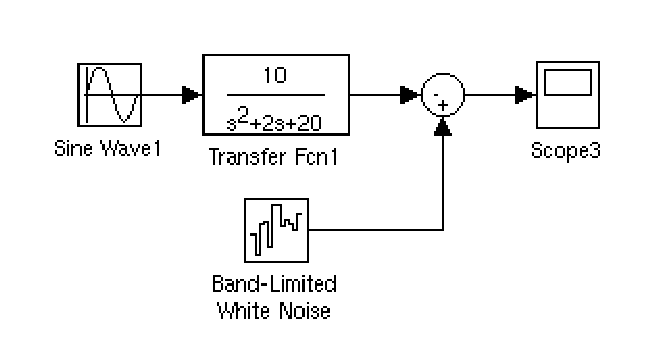
\includegraphics[width=0.70\columnwidth]{figures/sistema_ruido.eps}
	\caption{Sistema em estudo sujeito ao efeito de ruido branco na sa�da do processo.}
	\label{fig:intro_sistema}
\end{figure}

